\chapter{The Screens}
As stated before, Little Sound Dj has several screens, laid out in a screen map of size \begin{math} 5 \times 3 \end{math}. You can
navigate between the screens by pressing \textsc{select+cursor}.
\section{Screen Map}
\begin{figure}[htbp]
\centering
\begin{tabular}{|c|c|c|c|c|l}

	\cline{0-4}
	\multicolumn{2}{|c|}{ } & & & &
	\\
	\multicolumn{2}{|c|}{Project} & Wave & Synth & &
	\\
	\multicolumn{2}{|c|}{ } & & & &
	\\
	\cline{0-3}
	& & & & & \\
	Song & Chain & Phrase & Instr. & Table  & \begin{math} \leftarrow \end{math} Main Row \\
	& & & & & \\
	\cline{0-4}
	\multicolumn{5}{|c|}{} \\
	\multicolumn{5}{|c|}{Groove} \\
	\multicolumn{5}{|c|}{} \\
	\cline{0-4}
\end{tabular}
%\caption{Screen Map.}
\end{figure}

The song, chain and phrase screens are used for sequencing and arranging. The wave, synth,
instrument and table screens are used for sound programming. \footnote{There are also three hidden
screens, not shown on the map: The file, word and help screens. We will get back to these later.}

The remaining screens, project and groove, have more general purposes. The bulk of your activities will however probably be in the so-called "main row," in the middle of the map, as that's where the composing is done.

\section{Starting and Stopping}

When pressing \textsc{start} in the song screen, Little Sound Dj will always try to play all four
channels. When pressing \textsc{start} in the other screens, Little Sound Dj will only try to play the
channel that's indicated in the three-letter field at the right edge of the screen (\textsc{pu1}, \textsc{pu2}, \textsc{wav} or \textsc{noi}).

If you want to start playing all four channels from some other screen than the song screen,
you can do that by pressing \textsc{select+start}.

\section{Song Screen}

\begin{figure}[hbtp]
\centering
\fbox{ 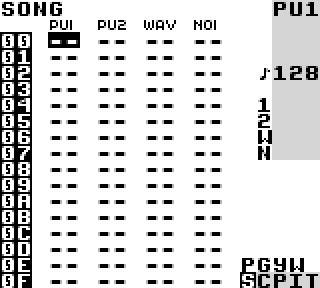
\includegraphics{song} }
\caption{Song Screen}
%\label{fig:song}
\end{figure}

The song screen
%(figure~\ref{fig:song})
is the highest level of the sequencer. This is where you arrange your songs.

The screen contains four columns, one for each channel. The columns contain lists of chains, which will be played from top to down. Different chains are used for different channels.

To insert a chain, move the cursor to an empty step and press \textsc{a}. If you want to add a new
chain, press \textsc{a} twice. To edit a chain, move the cursor to the chain number and press
\textsc{select+right}. To remove a chain, you can either press \textsc{a} twice or
press \textsc{b+a}.

To start or stop playing all channels in the song screen, press \textsc{start}. To instantly re-start all channels in the song screen, press \textsc{select+start} (this has the same effect as pressing \textsc{start, start} quickly).


\includegraphics[width=1cm]{tip}TIP!
\begin{itemize}
\item \textit{You can pull up down-below chains by pressing \textsc{b+a} on an empty step.}
\item \textit{\textsc{b+up/down} does page up/down.}
\item \textit{You can add or remove song screen bookmarks by tapping \textsc{b} three times \textsc{(b, b, b)}. This will shade the area under the cursor.}
%	\marginpar{
\includegraphics[width=1cm]{tip}TIP!}
\end{itemize}

The number of rows in the song screen is limited to 255 (\$00-\$FE).

\section{Chain Screen}
Chains are used for stringing phrases together, thus creating a unit built out of many
phrases. A chain can represent a longer rhythm block, a melody or a bass line.

The chain screen contains two columns. The first column contains the list of phrases that are
to be stringed together, while the second column transposes the phrase on the same row.

\begin{figure}[hbtp]
\centering
\fbox{ 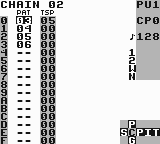
\includegraphics{chainexample} }
\caption{Chain Screen}
\label{fig:chainexample}
\end{figure}

Example:
The chain in figure~\ref{fig:chainexample} would play phrase 3, adding 5 semitones to each note, and then play each of the phrases 4, 5, 6, without transposing.

To add a phrase to the chain, move the cursor to an empty step and press \textsc{a}. If you want to
insert a new phrase, press \textsc{a} twice. To edit a phrase, move the cursor to the phrase number
and press \textsc{select+right}.

When editing a chain, you can go to the chain in a neighboring channel by pressing \textsc{b+left/right}. It is also possible to go to the next or previous chain in the song screen by
pressing \textsc{b+up/down}.

The different channels all share the same set of chains; that is, no chain is ever assigned to a
specific channel. The number of chains is limited to 128 (\$00-\$7F).

\section{Phrase Screen}

\begin{figure}[hbtp]
\centering
\fbox{ 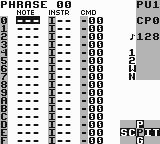
\includegraphics{phrase} }
%\caption{Phrase Screen}
%\label{fig:phrase}
\end{figure}

The phrase screen is where you enter notes. It has four columns: note, instrument, command and command value.

Phrases are shared between channels; that is, any phrase may be played back on any channel. A phrase might however sound very different depending on which channel it is played back on. As an example, if a phrase plays a melody using a pulse instrument, it will probably sound good in the pulse channels but strange in the other channels.

The note column looks different depending on instrument. Usually it shows note and octave, but instruments that play back samples (\textsc{kit}, \textsc{speech}) show sample names instead.

The instrument column selects instrument. There are 65 instruments in total, all of which can be changed in the instrument screen.


\includegraphics[width=1cm]{tip}TIP!
\begin{itemize}
    \item \textit{Notes without instrument change pitch or sample without a retrig.}
\end{itemize}

The command column is used to add effects. For example, the K command kills the sound of the channel.

There are 255 phrases (\$00-\$FE). The number of the phrase being edited is shown in the top of the screen.


\includegraphics[width=1cm]{tip}TIP!
\begin{itemize}
    \item \textit{Phrases are 16 steps by default. To shorten the length, use the H (hop) command.}
    \item \textit{Mute kit note columns by pressing \textsc{a+right} until \textsc{off} appears.\footnotemark}
        \footnotetext{Only works for kits with fewer than 15 samples.}
\end{itemize}


\section{Instrument Screen}

\begin{figure}[hbtp]
\centering
\fbox{ 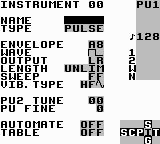
\includegraphics{instr-pulse} }
\caption{Instrument Screen}
\label{fig:instr2}
\end{figure}

There are five types of instruments available:

\begin{description}
\item[\textsc{pulse}] This instrument type produces pulse waves, and is used in pulse channels 1 and 2.
\item[\textsc{wave}] This instrument type can play back waves synthesized using the synth screen. It is used in the wave channel.
\item[\textsc{kit}] This instrument type plays sampled kits, stored in \textsc{rom}. (The samples are stored in 4 bits, 11,468 kHz.) It is used in the wave channel.
\item[\textsc{noise}] This instrument type produces filtered noise, and is used in the noise channel.
\item[\textsc{speech}] This instrument is locked to instrument number \$40, and is used for programming speech. For learning how to generate speech, please read chapter \ref{speech-chapter}.
\end{description}

You can change the instrument type by going to the type row and pressing \textsc{a+cursor}.

Remember that instruments don't automatically play in the right channel. For example, if you want to use a kit instrument to play drum samples, you have to do the following:

\begin{enumerate}
\item Go to the song screen, move cursor to the wave column, and insert a new chain by tapping \textsc{a} twice.
\item	Edit the chain by pressing \textsc{select+right}.
\item	Insert a new phrase by tapping \textsc{a} twice.
\item	Edit the phrase by pressing \textsc{select+right}. Now, you have a new phrase that is mapped to the wave channel.
\item	Create a new instrument by moving the cursor to the instrument column and tapping \textsc{a} twice.
\item	Press \textsc{select+right} to edit the instrument.
\item	Change the instrument type to \textsc{kit}.
\item	Go back to the phrase screen to start using your new instrument.
\end{enumerate}


\includegraphics[width=1cm]{tip}TIP!
\begin{itemize}
	\item \textit{In the instrument screen, press \textsc{select+b} to copy instruments and \textsc{select+a} to paste.}
%\marginpar{
\includegraphics[width=1cm]{tip}TIP!}
\end{itemize}

\subsection{General Instrument Parameters}
\label{general-instrument-parameters}

These parameters are used in most instrument types.

\begin{description}
	\item[\textsc{name}] Name the instrument by pressing \textsc{a}. This is useful for keeping track of your instruments. The instrument name will also be shown in the border when selecting instruments in the phrase screen.
	\item[\textsc{type}] Instrument type.
	\item[\textsc{length}] Sound length.
	\item[\textsc{output}] Send the sound to left/right/both/none speakers. (Use the headphone output to hear the difference!)
    \item[\textsc{pitch}] Controls the behavior of \textsc{p}, \textsc{l} and \textsc{v} commands. \textsc{A+u/d} switches pitch update speed: \textsc{fast} updates pitch at 360 Hz; \textsc{tick} updates pitch every tick; \textsc{step} is like \textsc{fast} except that \textsc{p} does pitch change instead of pitch bend; \textsc{drum} is like \textsc{fast} with logarithmic pitch, useful for \textsc{p} kicks. \textsc{a+l/r} changes vibrato shape between downwards triangle, saw and square, and upwards triangle, saw and square.
    \item[\textsc{transp.}] When \textsc{on}, the pitch may be affected by project and table transposes.
    \item[\textsc{cmd/rate}] Slows down \textsc{c} and \textsc{r} commands.
        Also affects \textsc{p} and \textsc{v} commands when \textsc{pitch} is set to \textsc{tick}.
        0=fastest, F=slowest.
    \item[\textsc{table}] Selects a table to run when playing notes. To edit the table, press \textsc{select+right}. To create a new table, press \textsc{a,a}. To clone the table, press \textsc{select+(b,a)}.
        Changing \textsc{play} to \textsc{step} makes Little Sound Dj step through the table, advancing one step every time the instrument is triggered.
\end{description}

\subsection{Pulse Instrument Parameters}
\label{detune}

\begin{figure}[htpb]
	\begin{center}
\fbox{ 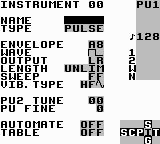
\includegraphics{instr-pulse} }
	\end{center}
	\caption{Pulse Instrument Screen}
	\label{fig:instr-pulse}
\end{figure}

\begin{description}
	\item[\textsc{envelope}] The first digit sets initial amplitude (0-\$F); the second digit sets release (0, 8: none, 1-7: decrease amplitude, 9-\$F: increase amplitude).
	\item[\textsc{wave}] Choose the wave type to be used.
	\item[\textsc{sweep}] Modulate the frequency. This only works on pulse channel 1. See Sweep/Shape (\textsc{s}) command documentation for further information.
\end{description}

The finetune settings create interesting phase effects when the same phrase is played on both pulse channels:

\begin{description}
	\item[\textsc{pu2 tsp.}] Transpose pulse channel 2.
	\item[\textsc{finetune}] Detune pulse channel 1 downwards, channel 2 upwards.
\end{description}

\subsection{Wave Instrument Parameters}

The wave instrument can play back synth sounds generated by the soft synthesizer found in the \textsc{synth} screen.

\begin{figure}[hbtp]
	\begin{center}
		\fbox { 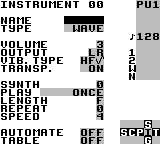
\includegraphics{instr-wave} }
	\end{center}
	%\caption{Wave Instrument Screen}
	%\label{fig:instr-wave}
\end{figure}

\begin{description}
	\item[\textsc{volume}] Set amplitude (0=0\%, 1=25\%, 2=50\%, 3=100\%)
	\item[\textsc{synth}] Select the synth sound to play back. To edit the synth sound being used, press \textsc{select+up} to go to the \textsc{synth} screen. If you want to use a new synth, tap \textsc{a} twice.
	\item[\textsc{play}] How to play back the synth sound: Once, loop, pingpong loop or manual. By selecting manual, only the first wave in the synth sound will be played, allowing you to step through the sound manually using the \textsc{f} command.
	\item[\textsc{length}] Set the length of the synth sound.
	\item[\textsc{repeat}] Set the loop point of the synth sound.
	\item[\textsc{speed}] Set how fast the synth sound should be played back.
\end{description}

\subsection{Kit Instrument Parameters}

\begin{figure}[hbtp]
	\begin{center}
	\fbox {	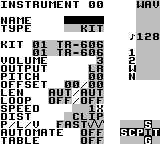
\includegraphics{instr-kit} }
	\end{center}
	%\caption{Kit Instrument Screen}
	%\label{fig:instr-kit}
\end{figure}

\begin{description}
	\item[\textsc{kit}] Choose the kits to use. The first kit will be used in the left note column in the phrase screen; the second kit will be used in the right note column in the phrase screen.
	\item[\textsc{pitch}] Pitch shift.
	\item[\textsc{offset}] Set the start loop point. If \textsc{loop} is set to \textsc{off}, this value can be used for skipping the initial part of a sound.
	\item[\textsc{len}] Set the sound length. (\textsc{aut}=always play the sample to its end.)
	\item[\textsc{loop}] Loop the sample. (\textsc{off}=don't loop, \textsc{on}=loop sound and start playing from custom offset, \textsc{atk}=loop sample and start playing from the beginning.)
	\item[\textsc{speed}] Select full speed or half speed.
	\item[\textsc{dist}] Select the algorithm that should be used when two kits are mixed together. \textsc{clip} is the default type. \textsc{shape} and \textsc{shape2} sound similar to \textsc{clip}, but with more high frequencies and less bass. \textsc{wrap} can be used to add some interesting digital distortion. When pressing \textsc{a+(left, left)} while \textsc{clip} value is selected, the program will jump out of range and play back sound from raw memory when clipping.
\end{description}


\includegraphics[width=1cm]{tip}TIP!
\begin{itemize}
	\item \textit{For those running LSDj on emulator or with backup gear, there is a Java application for replacing the original sample kits available at} \url{http://littlesounddj.com/lsd/latest/lsd-patcher/}.
\end{itemize}

\subsection{Noise Instrument Parameters}
\label{noise-instrument-parameters}

\begin{figure}[htpb]
	\begin{center}
		\fbox { 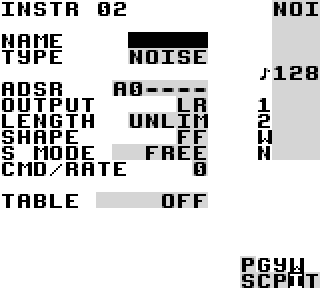
\includegraphics{instr-noise} }
	\end{center}
	\caption{Noise Instrument Screen}
	\label{fig:instr-noise}
\end{figure}

\begin{description}
	\item[\textsc{envelope}] First digit is initial amplitude (0-\$F); second digit is release (0, 8: none, 1-7: decrease amplitude, 9-\$F: increase amplitude).
    \item[\textsc{shape}] Noise generator control. The first digit changes pitch by octave, the second digit divides the frequency. Set the second digit to 0-7 for periodic noise, 8-\$F for random noise.
        For an in-depth technical explanation, refer to \href{https://google.com\&q=gbsound.txt}{gbsound.txt}.
	\item[\textsc{s mode}] When set to \textsc{free}, noise changing commands can randomly\footnotemark mute the sound. When set to \textsc{stable}, commands are limited so that sound will never be muted by accident.
\footnotetext{There is a 0.4\% risk that the sound gets muted when a shape that ends with digit 8-F
        is changed so that it ends with digit 0-7.}
\end{description}

\subsection{Speech Instrument Parameters}

For information about how to generate speech, please read chapter \ref{speech-chapter}.

The number of instruments is limited to 64 (hexadecimal: \$00-\$39).

\section{Table Screen}

Tables are sequences of transposes, commands and amplitude changes which can be executed at any speed and applied to any channel. By setting a table in the instrument screen, the table will start every time you play the instrument. This allows you to create more interesting sounds than would be possible using the instrument screen alone.

Tables contain six columns. The first column is the envelope column, used to create custom amplitude envelopes. Next is the transpose column, used to transpose the played note by a number of semitones. The other columns are command columns like the one in the phrase screen.

The default table speed of one tick per step can be changed using the G command.


\includegraphics[width=1cm]{tip}TIP!
\begin{itemize}
	\item \textit{The transpose column has special functionality when using \textsc{kit} or \textsc{noise} type instruments. For \textsc{kit}, the transpose column works as a pitch shifter. For \textsc{noise}, the transpose column works like the \textsc{s} (shape) command.}
\end{itemize}

\subsection{Custom Envelope Example}

The first digit in the envelope column sets the amplitude; the second digit sets for how many ticks that amplitude should remain.

\begin{figure}[htpb]
	\begin{center}
		\fbox{		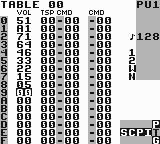
\includegraphics{table-amp} }
	\end{center}
	\caption{Table Envelope Example}
	\label{fig:table-amp}
\end{figure}

The table in figure~\ref{fig:table-amp} creates an amplitude envelope with short attack and medium sustain. It could be used for a bass instrument.

\subsection{Arpeggio Example}

\begin{figure}[htpb]
	\begin{center}
		\fbox{ 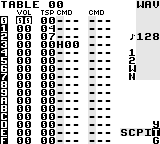
\includegraphics{table-arp}}
	\end{center}
	\caption{Arpeggio Example}
	\label{fig:table-arp}
\end{figure}

A typical use for tables is to create arpeggios. This is a musical term for playing notes very fast, so that the listener will get the impression that a chord is played. The table in figure~\ref{fig:table-arp} would emulate striking a major chord.

Shorter arpeggios can just as well be created using the C (chord) command in phrases (see \ref{command-chord} for example). Tables however still have to be used for creating longer arpeggios.

To view different tables, press \textsc{b+cursor}.


\includegraphics[width=1cm]{tip}TIP!
\begin{itemize}
	\item \textit{To give an instrument some attack, transpose the first table row a few steps up or down.}
	\item \textit{There is a shortcut between the phrase and table screens. Press \textsc{select+right} on an A command in the phrase screen to edit the table selected with the A command. To jump back, press \textsc{select+left}.}
\end{itemize}

The number of tables is limited to 32 (\$00-\$1F).

\section{Groove Screen}

Grooves define the speed by which your phrases and tables are played back. They can be used for giving your songs some extra swing. The different sound channels do not need to be synchronized to each other; this means that you can use a separate groove for each phrase and table.

\begin{figure}[htbp]
	\begin{center}
		\fbox{ 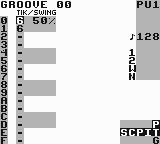
\includegraphics{groove} }
	\end{center}
	\caption{Groove Screen}
	\label{fig:groove}
\end{figure}

To understand grooves, you need to know that the sequencer's time handling is based on an abstract time period called \emph{tick}. The length of a tick varies with the song tempo; at 128 BPM, a tick is approximately 1/50th of a second. In the groove screen, you can specify for how many ticks each note step should be played.
The groove in figure~\ref{fig:groove} would make the sequencer spend approximately 6/50th of a second on every note step.

\begin{figure}[htbp]
	\begin{center}
		\fbox{ 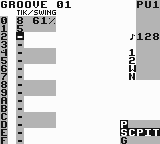
\includegraphics{groove-swing} }
	\end{center}
	\caption{Swing Example}
	\label{fig:groove-swing}
\end{figure}

You can also use the groove screen to create custom rhythms. The groove in figure~\ref{fig:groove-swing} would make the sequencer spend 8/50th of a second on even note steps, and 5/50th of a second on odd note steps, creating a swing. With thoughtful programming, grooves can also be used to create triplets and other complex rhythm structures.

Groove 0 is the default groove for all phrases. If you want to, you can easily switch to another groove using the groove (\textsc{g}) command in the phrase screen.

You can select the groove you wish to edit by pressing \textsc{b+cursor}.


\includegraphics[width=1cm]{tip}TIP!
\begin{itemize}
	\item \textit{ Pressing \textsc{a+up/down} will change the swing percentage, while keeping the total number of ticks -- and thus, the resulting song speed -- constant. (Example: Original value is 6/6 = 50\%. Press \textsc{a+up}. Now the value changes to 7/5 = 58\%!) }
	\item \textit{ If you switch to the groove screen when the cursor is on a \textsc{g} command in the phrase or table screens, Little Sound Dj will display the groove that is selected with the groove command.}
\end{itemize}

\section{Synth Screen}

The synth screen features a soft synthesizer that generates sounds to be played back by the wave instruments. In total, there are 16 synth programs. You can choose the program to edit by pressing \textsc{b+cursor}.

\begin{figure}[h]

\includegraphics[width=1cm]{tip}TIP!
\begin{itemize}
	\item \textit{Each synth program uses \$10 waves. Synth program 0 uses waves \$00-\$0F, synth program 1 uses waves \$10-\$1F, and so on. It is possible to look at the resulting synth sounds in the wave screen (Section~\ref{wave-screen-section}).}
\end{itemize}
\end{figure}

\begin{figure}[htbp]
	\begin{center}
		\fbox{		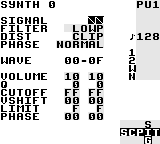
\includegraphics{synth}}
	\end{center}
	\caption{Synth Screen}
	\label{fig:synth}
\end{figure}

\subsection{General Parameters}

\begin{description}
\item[\textsc{signal}] Square, saw tooth or triangle.
\item[\textsc{filter}] Low-pass, high-pass, band-pass or all-pass.
\item[\textsc{dist}] Distortion mode. \textsc{Clip} truncates the wave to \textsc{limit}, \textsc{fold} mirrors the wave around \textsc{limit}, \textsc{wrap} wraps around vertically.
\item[\textsc{phase}] \label{phase}
Compress the waveform horizontally. It is applied after filtering with Q and cutoff. See figure \ref{fig:phasing} for examples.
\end{description}

\begin{figure}[hbtp]
	\centering
	\subfloat[Phase example. Original wave.]{
		\fbox{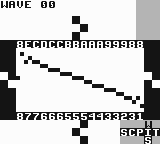
\includegraphics{phase-original}}
	}
	\qquad
	\subfloat[\textsc{normal} phasing. Compress horizontally, generate once.]{
	\fbox{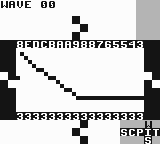
\includegraphics{phase-normal}}
	}

	\subfloat[\textsc{resync} phasing. Compress horizontally, loop.]{
		\fbox{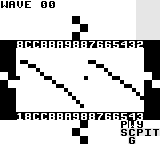
\includegraphics{phase-resync}}
	}
	\qquad
	\subfloat[\textsc{resyn2} phasing. Loop, but don't compress.]{
		\fbox{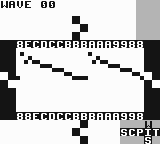
\includegraphics{phase-resyn2}}
	}
	\caption{Phase Examples}
	\label{fig:phasing}
\end{figure}

\subsection{Start and End Parameters}

Use these settings to specify values for the start and end of the sound. The program will then create a smooth fade between the start and end values.

\begin{description}
\item[\textsc{volume}] Signal volume.
\item[\textsc{q}] Resonance control. Boosts the signal around the cutoff frequency, to change how bright or dull the wave sounds.
\item[\textsc{cutoff}] Filter cutoff frequency.
\item[\textsc{vshift}] Shifts the signal vertically. See figure \ref{fig:vshift} for examples.
\item[\textsc{limit}] Limits the signal vertically using the \textsc{dist} mode.
\item[\textsc{phase}] 0 = no phase, \$1F = maximum phase. See figure \ref{fig:phasing} for examples.
\end{description}

\begin{figure}[htpb]
	\centering
	\subfloat[Vshift example. Original wave.]{
		\fbox{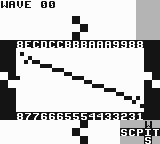
\includegraphics{vshift-original}}
	}

	\subfloat[Vshifted signal. Vshift = 40, clip = wrap.]{
	\fbox{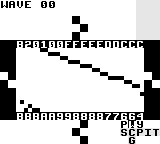
\includegraphics{vshift-40}}
	}

	\subfloat[Vshifted signal. Vshift = 80, clip = wrap.]{
		\fbox{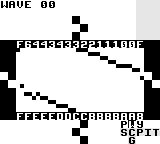
\includegraphics{vshift-80}}
	}
	\caption{Vshift Examples}
	\label{fig:vshift}
\end{figure}

\section{Wave Screen}
\label{wave-screen-section}

%\begin{figure}[htpb]
%	\begin{center}
%		\fbox{		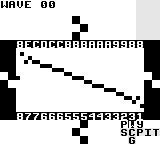
\includegraphics{wave}}
%	\end{center}
%	\caption{Wave Screen}
%	\label{fig:wave}
%\end{figure}
In the wave screen, you can view and edit the individual waveforms of the synth programs. There are 16 (\$10) synth programs, and each programs has \$10 waves. This means that synth sound 0 uses waves \$0-\$F, synth sound 1 uses waves \$10-\$1F, and so on.

To change selected values, press \textsc{up/down}. To flip selected values, press \textsc{a+cursor}. \textsc{B+cursor} navigates between different waves.

It is possible to modify multiple values at once, using the regular key presses:

\begin{description}
	\item[\textsc{select+b}] Start selection.
	\item[\textsc{select+b,b}] Select the entire wave.
	\item[\textsc{b}] Copy selection to clipboard.
	\item[\textsc{up/down}] Move selection up/down.
	\item[\textsc{a+left/right}] Flip selection horizontally.
	\item[\textsc{a+up/down}] Flip selection vertically.
	\item[\textsc{select+a}] Paste from clipboard.
\end{description}

\section{Project Screen}

\begin{figure}[htpb]
	\begin{center}
		\fbox{		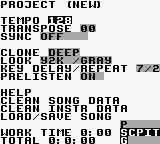
\includegraphics{project}}
	\end{center}
	\caption{Project Screen}
	\label{fig:project}
\end{figure}

The project screen (figure~\ref{fig:project}) contains settings that affect the entire program.

\begin{description}
	\item[\textsc{tempo}] Change the tempo. It is possible to set a new tempo either by pressing
\textsc{a+cursor}, or by tapping the \textsc{a} button in pace with the desired tempo. When being
slave in sync mode, it is possible to temporarily play a little faster or slower by pressing \textsc{a+left/right}.
	\item[\textsc{transpose}] Adjust the pitch of the pulse and wave instruments, by a given number of semitones.
	\item[\textsc{sync}] Activate link-up over the serial port. (Read more about this in chapter \ref{sync-chapter}!)

	\item[\textsc{clone}] Select deep or slim chain cloning. Deep chain cloning will also clone the phrases of a chain when cloning, whereas slim cloning will re-use the old phrases. Read chapter 3 for a full explanation of cloning.
	\item[\textsc{look}] Change the font and color set.
	\item[\textsc{key delay/repeat}] Set repeat delay and repeat rate of the Game Boy buttons.
	\item[\textsc{prelisten}] Play notes and instruments while entering them.

	\item[\textsc{help}] Enter help screen. The help screen contains a quick reference for button presses and a command list.
	\item[\textsc{clean song data}] Clear all phrases and chains that are not used in the song. Also, if there are several phrases with the same content, they will be reduced to one. \label{clean-song-data}
	\item[\textsc{clean instr data}] Clear all instruments, tables, synths and waves that are not used in the song.
	\item[\textsc{load/save song}] Enter file manager. \footnote{The file manager is only available for cartridges that have 1 Mbit SRAM or more. In case your cartridge doesn't have 1 Mbit SRAM, this button will be replaced with a \textsc{reset memory} button.}
\end{description}

This screen also contains two clocks. The \textsc{work time} clock displays the time Little Sound Dj has been used since the last memory reset, in hours and minutes. When playing, the clock
is replaced by a \textsc{play time} clock, which shows for how long the song has been playing. The \textsc{total} clock displays the time Little Sound Dj has been used in total, in days, hours and minutes.

\subsection{Total Memory Reset}
\label{total-memory-reset}

It is possible to reset the cartridge by pressing \textsc{select+a+b} on \textsc{load/save file}. This will erase all songs and bring back the cartridge to its default state. This can be useful if memory got scrambled, or if you want to erase all songs quickly.

\section{File Screen}

\begin{figure}[htpb]
	\begin{center}
		\fbox{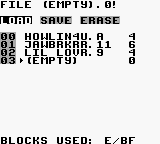
\includegraphics{file}}
	\end{center}
	\caption{File Screen}
	\label{fig:file}
\end{figure}

The file screen (figure~\ref{fig:file}) is entered by pressing the \textsc{load/save file} button in the project screen. The file screen is used for saving the song you are working on to the storage memory. It can also be used to load songs from the storage memory to the work memory. The file screen allows you to keep up to 32 songs on one cartridge.

\textsc{Note}: The file screen is only available for cartridges that have 1 Mbit SRAM or more.

\begin{description}
	\item[\textsc{file}] Shows the file name of the song you are working on. The exclamation mark (\textsc{!}) indicates when changes have been made to a song.
	\item[\textsc{load}] Load a song. Press \textsc{a}, select the file to load and press \textsc{a} again.
	\item[\textsc{save}] Save song. Press \textsc{a}, select the slot to save to and enter the file name.
	\item[\textsc{del}] Delete a song. Press \textsc{a}, select the file to delete and press \textsc{a} again.
	\item[\textsc{blocks used}] Shows how much of the storage memory that is used. One block equals 512 bytes. The digits on the bottom are hexadecimal, meaning there is a total of \$BF * 512 = 97,792 available bytes.
\end{description}

If you want to cancel an operation in this screen, simply press \textsc{b}.

\begin{figure}[hbtp]

\includegraphics[width=1cm]{tip}TIP!
\begin{itemize}
        \item \textit{There is a useful file manager application available at} \url{http://littlesounddj.com/lsd/latest/lsd-manager/}.
	\end{itemize}
\end{figure}

\subsection{Song List}

The song list presents song name, version number and file size. When saving, the song is compressed, so the resulting file size will vary with different songs. If you want to start a new project, load from the \textsc{(empty)} slot.


\includegraphics[width=1cm]{tip}TIP!
\begin{itemize}
    \item{While in the song list, it is possible to press \textsc{select+a} to load a song without switching to the song screen, and \textsc{start} to start/stop songs. In this way, you can load and play songs without jumping back and forth between screens. This can be handy if you are playing a live show with prepared tracks and want fewer things to think about.}
\end{itemize}

\section{Border Information}

A lot of useful data is displayed in the screen border (figure~\ref{fig:border}).

\begin{figure}[htpb]
	\begin{center}
	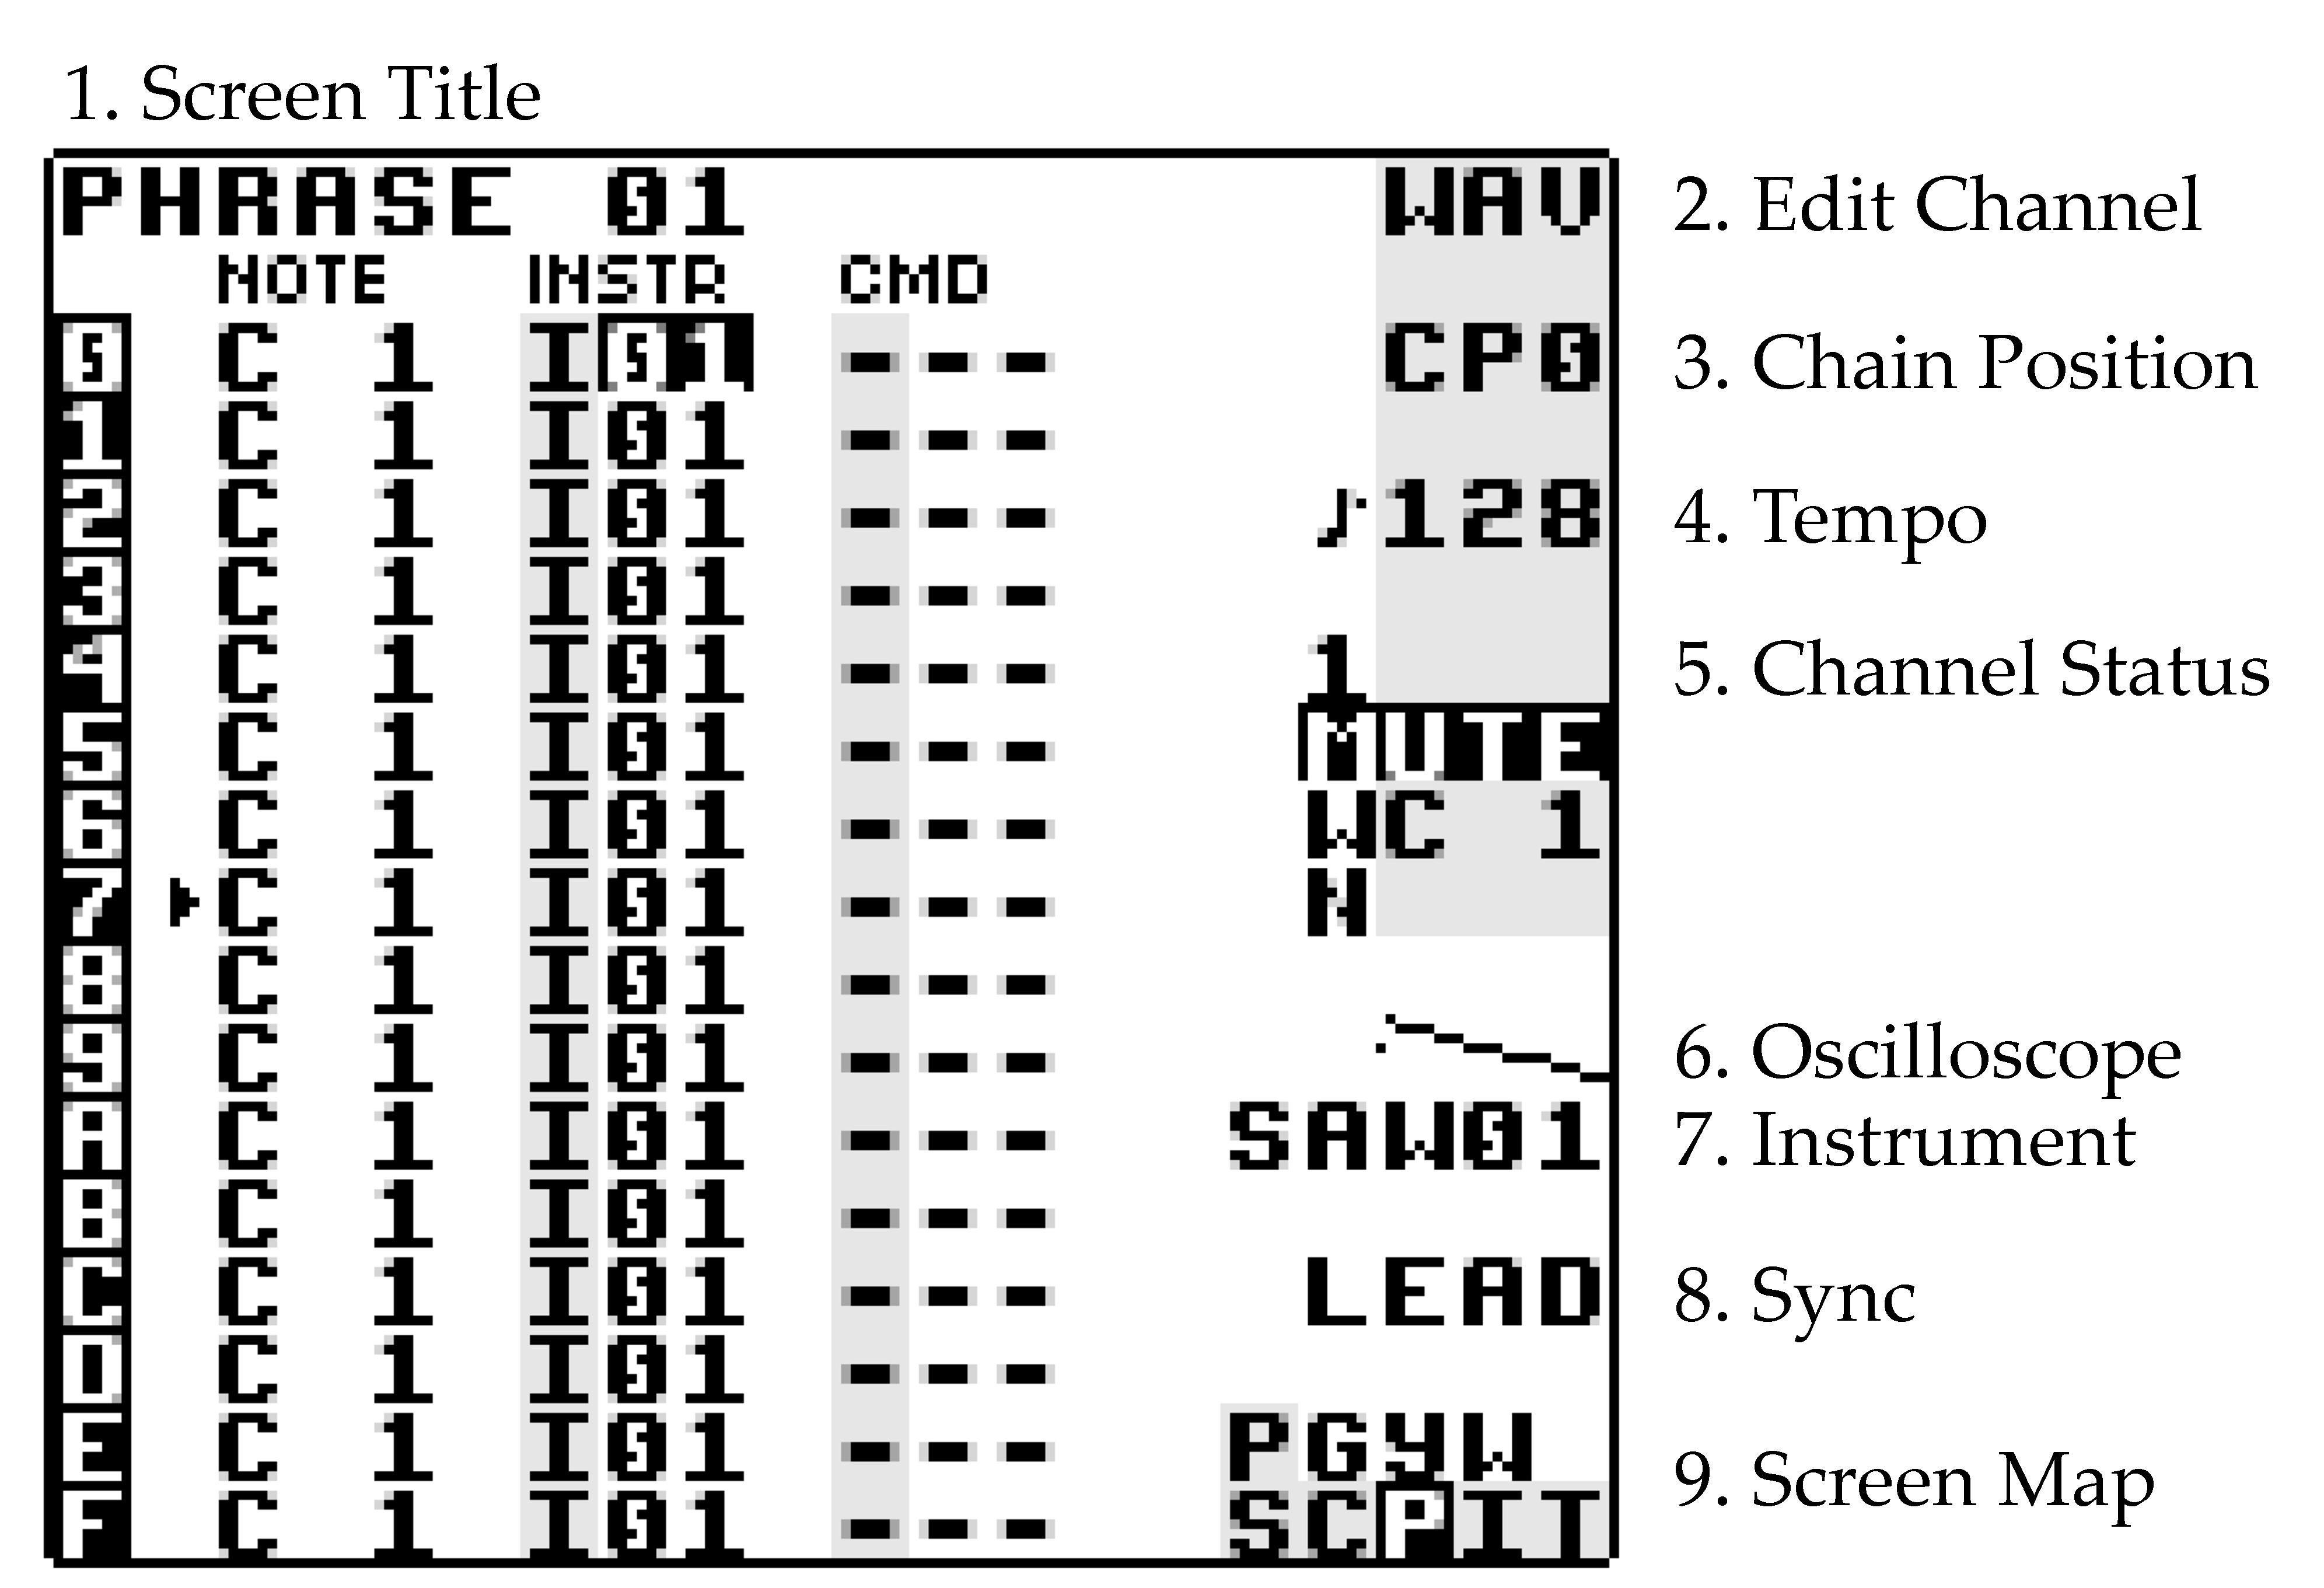
\includegraphics[width=12cm]{border}
	\end{center}
	\caption{Border Information}
	\label{fig:border}
\end{figure}

\begin{enumerate}
\item Screen name.
\item Phrase/chain/instrument/table/frame/groove number.
\item Active channel.
\item Chain position being edited.
\item Current tempo, in beats per minute (\textsc{bpm}).
\item Notes being played.
\item Sync information.
\item Mute. (The characters will be lit when pressing \textsc{b+select} or \textsc{b+start}.)
\item Screen map.
\end{enumerate}


